\documentclass{beamer}  
%导言区
%\usepackage[UTF8,noindent]{ctexcap}%阻止ctex宏包引入的短浅缩进
\usetheme{AnnArbor}
\usepackage{graphicx}
%set equation theme
\setbeamertemplate{footline}[frame number]{}
\usefonttheme{professionalfonts}
\usepackage{algorithm2e}
\usepackage{algorithmic}
\usepackage[level]{datetime} 
\usepackage{biblatex}
	\bibliography{BMVC2018}

%set theme
\useinnertheme{rectangles}
\useoutertheme{smoothbars}%sidebar
\usecolortheme{crane}%crane
\begin{document}  
	
%second section 
	
	
	\title{High-Resolution Image Synthesis and Semantic Manipulation with Conditional GANs}
	\institute[SCUT]{South China University of Technology}
	%\logo{
\includegraphics[height=0.45\textwidth]{graphics/scut.pdf}}
	\author{Presented by Junhong Huang}
	\titlegraphic{	
\includegraphics[height=0.35\textwidth]{images/scut.pdf}}
	\date{May 27, 2018, SAIL}
	\keywords{GAN,WGAN,machine learning,deep learning}
	
	%first
	\begin{frame}
	\maketitle
\end{frame}

\begin{frame}{Contents}
%content
\tableofcontents
\end{frame}



\AtBeginSection[]
{
\begin{frame}{Contents}

\tableofcontents[currentsection]

\end{frame}
}

\section{Motivation}
\begin{frame}{Motivation}{High-Resolution Image Synthesis \& Semantic Manipulation }
\begin{figure}
	\centering
	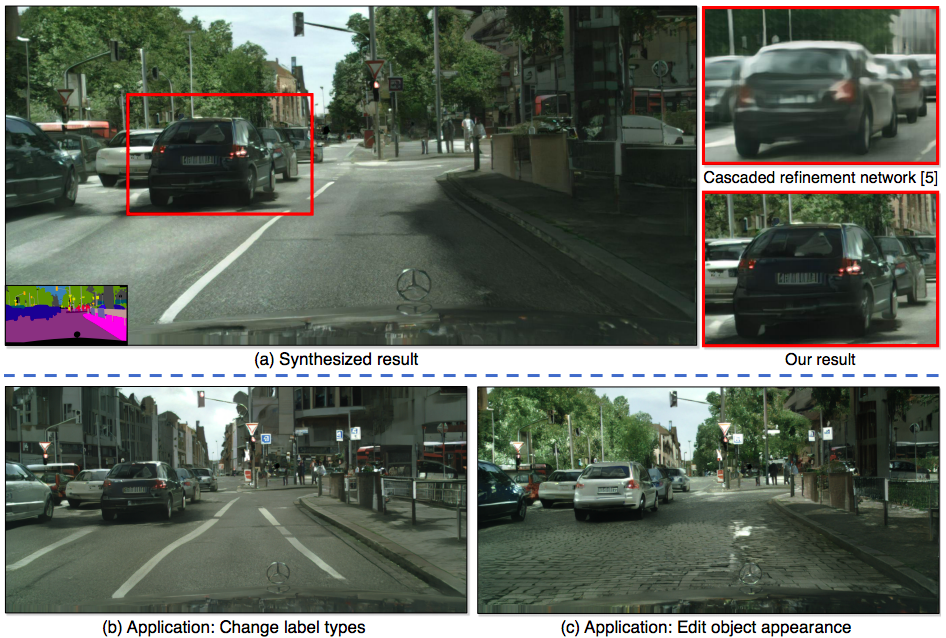
\includegraphics[height=0.5\textheight]{images/conclusion}
%	\caption{$2048\times1024$ images generated from the  semantic label map (lowe left coner in (a))}
\end{figure}
\setbeamercolor{uppercol}{fg=white,bg=blue!75!black}%
\setbeamercolor{lowercol}{fg=black,bg=blue!20}%
\begin{beamerboxesrounded}[upper=uppercol,lower=lowercol,shadow=false]{In this paper,}
	\begin{itemize}
	\item
	high-resolution image synthesis is \textbf{generating $2048\times1024$ photo-realistic images} from semantic label maps;
	\item
	semantic manipulation means allowing users to \textbf{edit the object appearance} interactively.
	\end{itemize}
\end{beamerboxesrounded}
\end{frame}

\section{Method}
\begin{frame}{The pix2pix Baseline \footcite{Image-to-image translation with conditional adversarial networks (CVPR 2017)}}
\begin{figure}
	\centering
	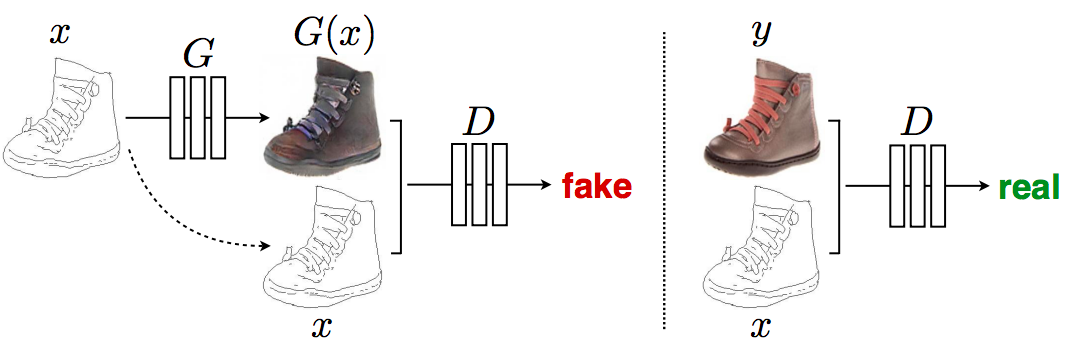
\includegraphics[height=0.45\textheight]{images/baseline}
\end{figure}
\end{frame}

\begin{frame}{Improving Photorealism and Resolution}{Coarse-to-Fine Generator}
	\begin{figure}
	\centering
	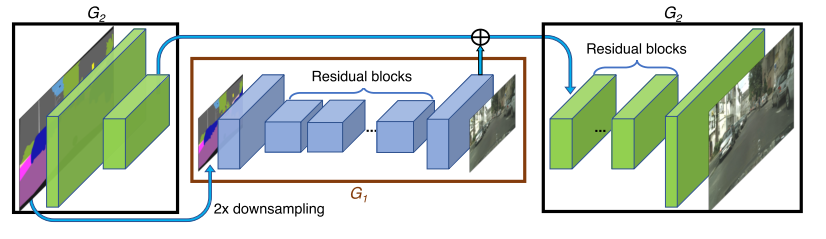
\includegraphics[height=0.4\textheight]{images/structure}
\end{figure}
\end{frame}

\begin{frame}{Improving Photorealism and Resolution}{Multi-scale  Discriminators}

\end{frame}

\begin{frame}{Using Instance Maps}
\begin{figure}
	\centering
	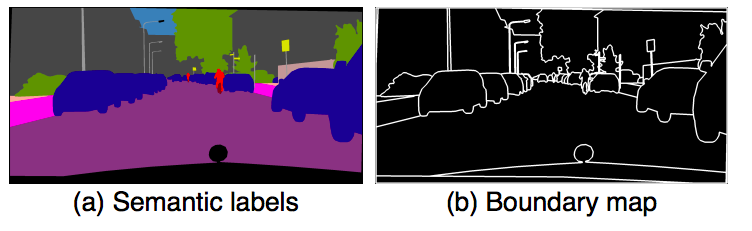
\includegraphics[height=0.45\textheight]{images/instance_maps}
\end{figure}
\begin{figure}
	\centering
	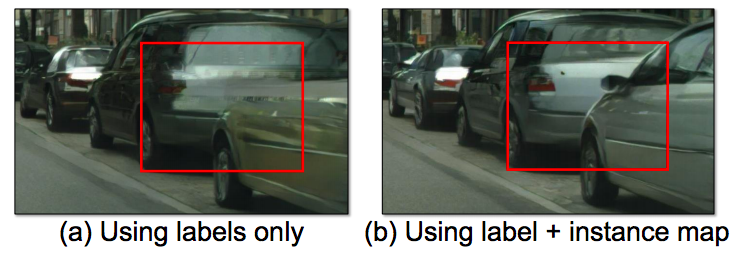
\includegraphics[height=0.45\textheight]{images/instance_result}
\end{figure}
\end{frame}

\begin{frame}{Learning an Instance-level Feature Embedding}
\begin{figure}
	\centering
	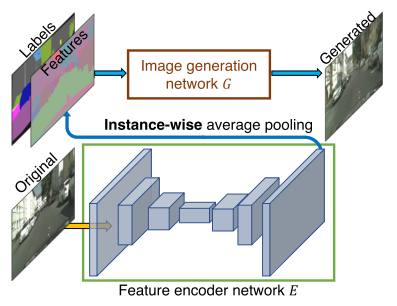
\includegraphics[height=0.6\textheight]{images/instance}
\end{figure}
\end{frame}







\section{Experimental Results}
\begin{frame}{Datasets and Baselines}
\setbeamercolor{uppercol}{fg=white,bg=blue!75!black}%
\setbeamercolor{lowercol}{fg=black,bg=blue!20}%
\begin{beamerboxesrounded}[upper=uppercol,lower=lowercol,shadow=false]{In this paper, }
	\begin{itemize}
		\item
	datasets include \textbf{Cityscapes}, \textbf{NYU Indoor RGBD}, \textbf{ADE20K} and \textbf{Helen Face} datasets;
		\item
	baselines contain \textbf{pix2pix} \footcite{Image-to-image translation with conditional adversarial networks (CVPR 2017)} and \textbf{CRN} \footcite{Photographic image synthesis with cascaded refinement networks (ICCV 2017)}
	\end{itemize}
\end{beamerboxesrounded}
\end{frame}

\begin{frame}{Quantitative Comparisons }
\begin{figure}
	\centering
	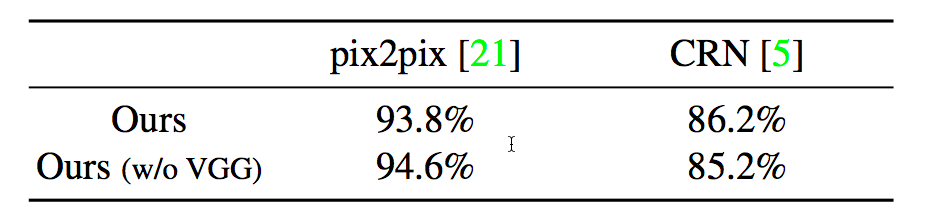
\includegraphics[height=0.3\textheight]{images/quantitative}
\end{figure}
\end{frame}


\begin{frame}{Human Perceptual Study}{Unlimited Time}
\begin{figure}
	\centering
	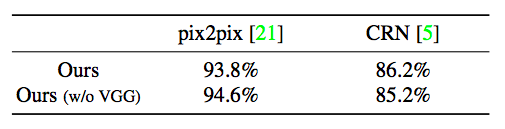
\includegraphics[height=0.35\textheight]{images/unlimite_time}
\end{figure}
\end{frame}

\begin{frame}{Human Perceptual Study}{Unlimited Time}
\begin{figure}
	\centering
	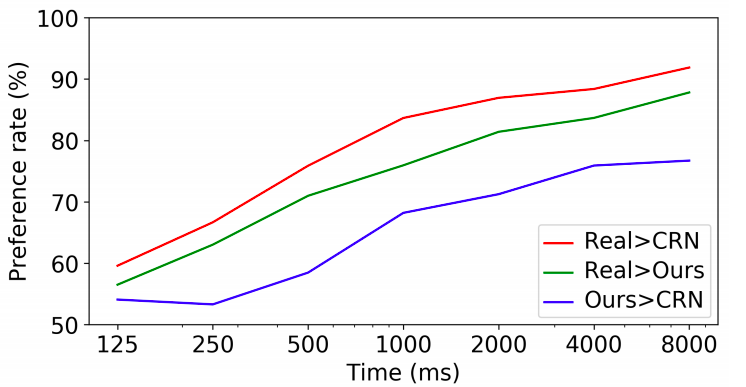
\includegraphics[height=0.45\textheight]{images/limite_time}
\end{figure}
\end{frame}

\begin{frame}{Analysis of Proposed Model}{Analysis of The Loss Function}
\begin{figure}
	\centering
	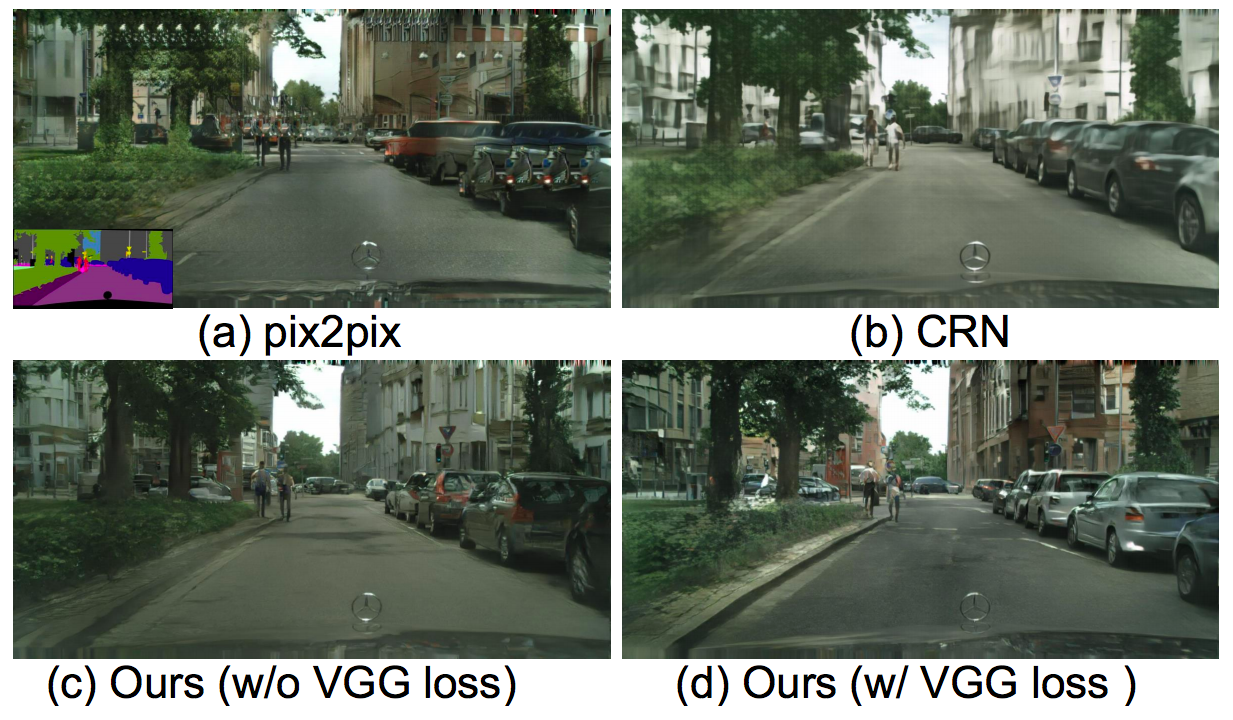
\includegraphics[height=0.8\textheight]{images/result_1}
\end{figure}
\end{frame}


\begin{frame}{Analysis of Proposed Model}{Analysis of The Loss Function}
\begin{figure}
	\centering
	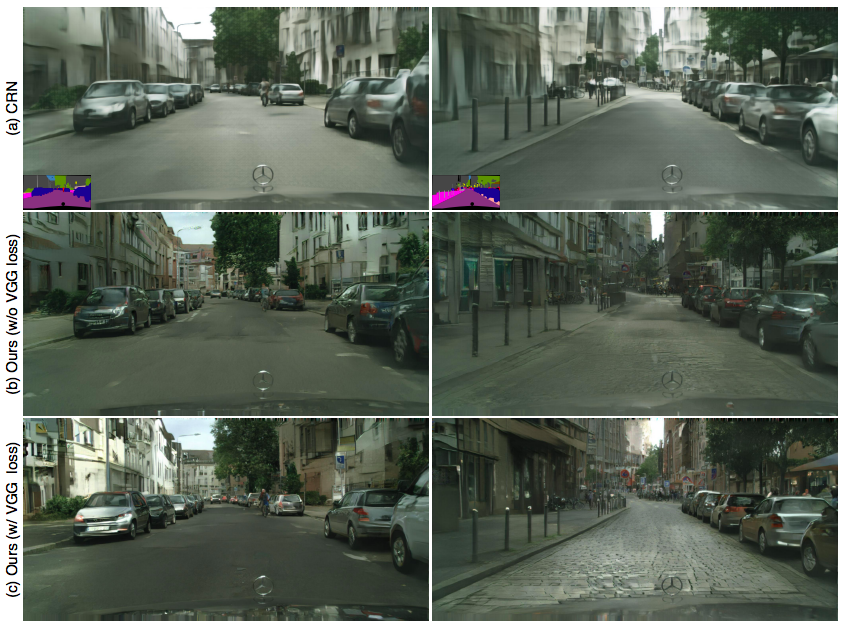
\includegraphics[height=0.8\textheight]{images/result_3}
\end{figure}
\end{frame}

\begin{frame}{Analysis of Proposed Model}{Analysis of  Using Instance Maps}

\end{frame}

\begin{frame}{Analysis of Proposed Model}{Analysis of  The generator}
\begin{figure}
	\centering
	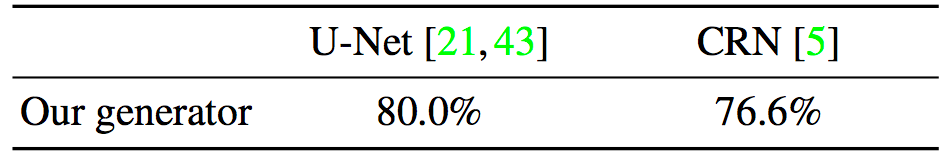
\includegraphics[height=0.2\textheight]{images/table_3}
\end{figure}
\end{frame}

\begin{frame}{Analysis of Proposed Model}{Analysis of The Discriminator}
\begin{figure}
	\centering
	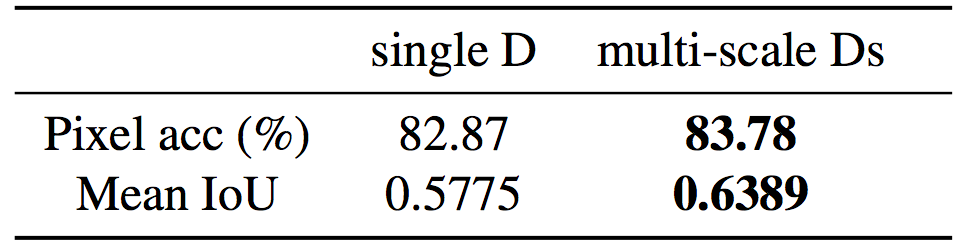
\includegraphics[height=0.3\textheight]{images/table_4}
\end{figure}
\end{frame}

\begin{frame}{Iterative Object Editing}
\begin{figure}
	\centering
	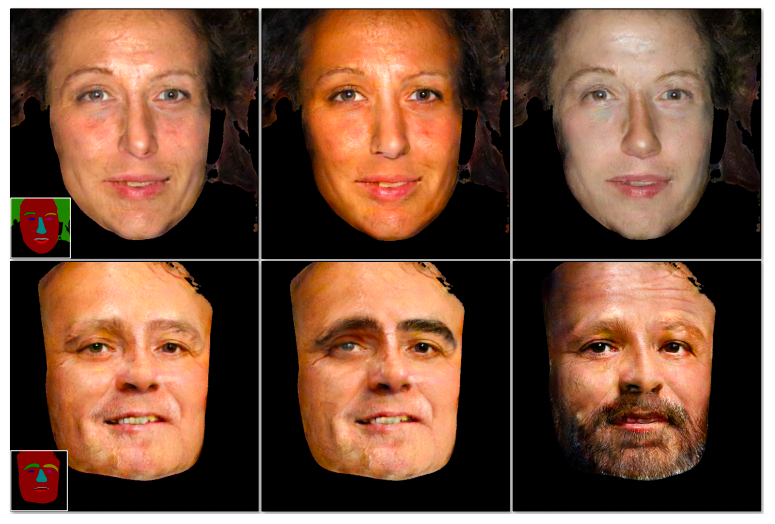
\includegraphics[height=0.6\textheight]{images/result_4}
\end{figure}
\end{frame}

\begin{frame}
	\begin{figure}
		\centering
		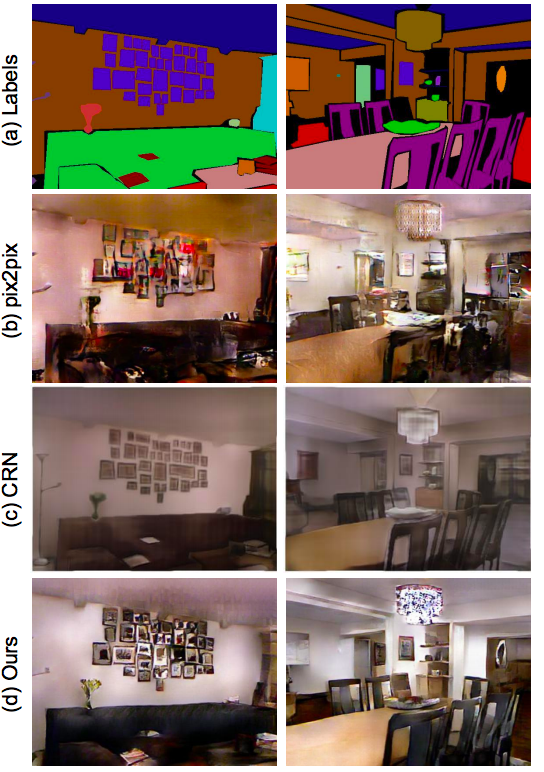
\includegraphics[height=0.9\textheight]{images/result_2}
	\end{figure}
\end{frame}





\section{Conclusions}

\end{document} 